\documentclass[conference]{IEEEtran}
\IEEEoverridecommandlockouts
\usepackage{cite}
\usepackage[spanish]{babel}
\usepackage{listings}
\usepackage{amsmath,amssymb,amsfonts}
\usepackage{algorithm}

\usepackage{algpseudocode}
\usepackage{graphicx}
\usepackage{textcomp}
\usepackage{xcolor}
\def\BibTeX{{\rm B\kern-.05em{\sc i\kern-.025em b}\kern-.08em
    T\kern-.1667em\lower.7ex\hbox{E}\kern-.125emX}}
\graphicspath{ {images/} }
\renewcommand{\spanishtablename}{Tabla}%renombrar tablas en español%
\begin{document}

\title{Practica 2 \\ Clasificación de frijoles mediante tecnicas de machine learning}

\author{\IEEEauthorblockN{1\textsuperscript{st} Erick Franco Gaona}
\IEEEauthorblockA{\textit{Departamento de Estudios Multidisciplinarios} \\
\textit{Universidad de Guanajuato}\\
Yuriria, México \\
e.francogaona@ugto.mx}
}

\maketitle

\begin{abstract}
Las regresiones se utilizan a menudo para predecir situaciones de la vida real en la industria y la ciencia. Existen diversas técnicas para realizar regresiones como pueden ser regresiones lineales multiples o bosques aleatorios. En este trabajo se presenta un caso de estudio de esas dos técnicas sobre un conjunto de datos público para revisar la diferencia de efectividad entre ambos métodos. Mientras que la regresión lineal multiple obtuvo un 82\% de efectividad, los bosques aleatorios obtuvieron un 88\% a costa de un mayor tiempo de ejecución.  
\end{abstract}

\section{Introducción}

La clasificación consta en ordenar u organizar las cosas en un conjunto de categorías o clases. Puedes categorizar ideas, objetos o cualquier tipo de referencia. El concepto de clasificación tiene diferentes vertientes: aprendizaje supervisado, no supervisado, semi supervisado y por refuerzo. El aprendizaje supervisado cuenta con un conocimiento a priori, es decir para la tarea de clasificar un objeto dentro de una categoría o clase se tienen modelos ya clasificados (objetos agrupados que tienen características comunes). En la primera fase se tiene un conjunto de entrenamiento o de aprendizaje (para el diseño del clasificador) y otro llamado de prueba o de validación (para clasificación), estos sirven para construir un modelo o regla general para la clasificación. En la segunda fase se clasifican los objetos o muestras de las que se desconoce la clase a las que pertenecen. 
A diferencia del aprendizaje supervisado, el aprendizaje no supervisado o clustering no se cuenta con conocimiento a priori, por lo que se tiene un área de entrenamiento disponible para la tarea de clasificación. En este tipo de clasificación contamos con “objetos” o muestras que tiene un conjunto de características, de las que no sabemos a qué clase o categoría pertenece, entonces la finalidad es el descubrimiento de grupos de “objetos” cuyas características afines nos permitan separar las diferentes clases. \\

En ocasiones, es muy complicado disponer de un conjunto de datos completamente etiquetado. Este tipo de aprendizaje tiene un poco de los dos anteriores. Usando este enfoque, se comienza etiquetando manualmente algunos de los datos. Una vez se tenga una pequeña porción de datos etiquetados, se entrena uno o varios algoritmos de aprendizaje supervisado sobre esa pequeña parte de datos etiquetados y se usan los modelos resultantes del entrenamiento para etiquetar el resto de los comentarios. Finalmente, se entrena un algoritmo de aprendizaje supervisado utilizando como etiquetas las etiquetadas manualmente y las generadas por los modelos anteriores. 
Por último, el aprendizaje por refuerzo es un método de aprendizaje automático que se basa en recompensar los comportamientos deseados y penalizar los no deseados. Es un aprendizaje que fija objetivos a largo plazo para obtener una recompensa general máxima y lograr una solución óptima. El juego es uno de los campos más utilizados para poner a prueba el aprendizaje por refuerzo. En estos casos, el agente recibe información sobre las reglas del juego y aprende a jugar por sí mismo. En un principio se comporta de manera aleatoria, pero con el tiempo empieza a aprender movimientos más sofisticados.  Este tipo de aprendizaje se aplica también en otras áreas como la robótica, la optimización de recursos o sistemas de control.\\

En este trabajo se cuenta con un dataset público que posee 16 características de 6 diferentes tipos de frijol, por lo que, se utiliza el aprendizaje supervisado. En las siguientes secciones se explica la teoria y ejemplifica mediante el caso de estudio su aplicación. 

\section{Teoría}
\subsection{Clasificador bayesiano simple}
El teorema de Bayes es utilizado para calcular la probabilidad de un suceso, teniendo información de antemano sobre ese suceso. Es posble calcular la probabilidad de un suceso A, sabiendo además que ese suceso cumple cierta característica que condiciona su probabilidad. El teorema de la probabilidad total hace inferencia sobre un suceso B, a partir de los resultados de los sucesos A. Por su parte, Bayes calcula la probabilidad de A condicionado a B. Para calcular la probabilidad tal como la definió Bayes en este tipo de sucesos, es necesaria la siguiente fórmula: 

\begin{equation}
P[A_n/B]= \frac{P[B/A_n]*P[A_n]}{\sum P[B/A_i]*P[A_i]}
\end{equation}

donde B es el suceso sobre el que se tiene información previa y $A_n$ son los distintos sucesos condicionados. En la parte del numerador se encuentra la probabilidad condicionada, y el denominador la probabilidad total. \\
\\
Los clasificadores NaiveBayes (NBC por sus siglas en inglés) son algoritmos de aprendizaje automático simples pero potentes. Se basan en la probabilidad condicional y el teorema de Bayes. SE deben seguir los siguientes pasos para implemntar el algoritmo: 
\begin{enumerate}
\item Convertir el conjunto de datos en una tabla de frecuencias
\item Crear una tabla de probabilidad calculando las correspondientes a que ocurran los diversos eventos o haciendo una distribución Gaussiana
\item La ecuación NaiveBayesse se usa para calcular la probabilidad posterior de cada clase
\item La clase con la probabilidad posterior más alta es el resultado de la predicción
\end{enumerate}

\subsection{Clasificación vecino más cercano (K-NN)}
El clasificador de vecinos más cercanos se basa en calcular las distancias entre el datoa  clasificar y los ejemplos de entrenamiento para decidir a que clase pertenece dependiendo de la menor distancia. No define de forma explícita una frontera de separación entre clases. La frontera se define implícitamente a partir de la distancia a las muestras del conjunto de entrenamiento. No requiere una representación de cada imagen en forma de vector, únicamente la definición de una función de distancia entre dos imágenes. Se considera un método de lazy learning debido a que la generalización más allá de los datos de entrenamiento es demorada hasta que se hace una pregunta al sistema.\\

De igual forma, K vecinos más cercanos es uno de los algoritmos de clasificación más básicos y esenciales en Machine Learning. Pertenece al dominio del aprendizaje supervisado y encuentra una aplicación intensa en el reconocimiento de patrones, la minería de datos y la detección de intrusos. Este algoritmo consiste en seleccionar un valor de K vecinos. Al momento del análisis los K datos más cercanos al valor que se desea predecir será la solución. Acá lo importante es seleccionar un valor de K acorde a los datos para tener una mayor precisión en la predicción. Si k es muy pequeño el modelo será muy sensitivo a puntos que son atípicos o con ruido. Si K es muy grande el modelo tiende a asignar siempre la clase más grande.

\begin{algorithm}[H]
\caption{Clasificador vecinos cercanos NN}
\begin{algorithmic}
\Require \\D \Comment{datos de entrenamiento}\\
k \Comment{número de vecinos}\\
t \Comment{dato para clasificar}
\Ensure c \Comment{clase para clasificar t}
\State $N \gets 0$
\For{$d \in D$}
\If{$|N| \leq k$}
    \State $N=N \cup d_i$
\Else
    \If{$\exists \: u \in N$ tal que $sim(t,u) \geq sim(t,d)$}
    	\State $N=N-u$
    	\State $N=N\cup d_i$
    \EndIf
\EndIf
\EndFor
\State $c=$ clases para los mejores $u \in N$ que son clasificados 
\end{algorithmic}
\end{algorithm}

Para el calculo de la distancia entre los vecinos se suelen utilizar la distancia euclidiana (ecuación 2) y distancia Manhattan (ecuación 3) siendo la primera la más común. La distancia euclidiana es un número positivo que indica la separación que tienen dos puntos en un espacio. La distancia entre dos puntos A y B de un espacio euclidiano es la longitud del vector AB perteneciente a la única recta que pasa por dichos puntos. Por otr lado, la distancia Manhattan dice que la distancia entre dos puntos es la suma de las diferencias absolutas de sus coordenadas. Es decir, es la suma de las longitudes de los dos catetos del triángulo rectangulo.

\begin{equation}
d_{ij}=\sqrt{\sum_{k=1}^{n}(x_{ki}-x_{kj})^2}
\end{equation}

\begin{equation}
d(p.q)=\sum_{i}^{n}|p_i-q_i|
\end{equation}

\subsection{Árboles de decisión}
La idea de la clasificación con árboles de decisión es simple: iterativamente se van generando particiones binarias (es decir de a dos agrupaciones) sobre la región de interés, buscando que cada nueva partición genere un subgrupo de datos lo más homogéneo posible. Primero se establece una condición. Dependiendo de si los datos cumplen o no la condición se tendrá una primera partición en dos subregiones. Y luego se repite el procedimiento anterior, una y otra vez, hasta que al final se obtengan agrupaciones lo más homogéneas posible, es decir con puntos que pertenezcan en lo posible a una sola categoría.\\

Para medir la homogeneidad se usa el índice Gini (ecuación 4), que mide el grado de impureza de un nodo: índices Gini iguales a cero indican nodos puros (es decir con datos que pertenecen a una sola categoría), mientras que índices mayores que cero y con valores hasta de uno indican nodos con impurezas (es decir con datos de más de una categoría). La entropía por su parte, es una medida que se aplica para cuantificar el desorden de un sistema (ecuación 5). Si un nodo es puro su entropía es 0 y solo tiene observaciones de una clase, pero si la entropía es igual a 1, existe la misma frecuencia para cada una de las clases de observaciones.
\begin{equation}
Gini(t)=1- \sum_{i}^{n}p_i^2
\end{equation}

\begin{equation}
H=- \sum_{i}^{n}p_i*\log_2p_i
\end{equation}

Los pasos para realizar un árbol de desición para clasificar son los siguientes: 
\begin{enumerate}

\item Para crear la raíz del árbol, es decir la primera partición, se toman todas las características y, para cada una de ellas, se definen todos los posibles umbrales a que haya lugar. Cada umbral será simplemente el punto intermedio entre dos valores consecutivos de cada característica.

\item Para cada uno de estos umbrales se calcula la partición (nodo izquierdo y nodo derecho) y para cada nodo hijo se calcula el índice Gini. Con estos nodos hijos se calcula la función de costo del nodo padre, que es el promedio ponderado de los índices Gini de sus hijos.

\item Se toma el umbral (o nodo padre resultante) que tenga la función de costo con el menor valor posible, indicando que la partición obtenida es la más homogénea de todas las analizadas.

\item Una vez se haya realizado esta partición, se repite el mismo procedimiento de forma iterativa para los nodos resultantes, exceptuando los que sean nodos hoja
\end{enumerate}

\subsection{Bosques aleatorios}
El bosque aleatorio tiende a combinar cientos de árboles de decisión y luego entrena cada árbol de decisión en una muestra diferente de las observaciones. Las predicciones finales del bosque aleatorio se realizan promediando las predicciones de cada árbol individual. El algoritmo de bosque aleatorio también puede ayudarte a encontrar características que son importantes en tu conjunto de datos. Esto se debe al algoritmo de Boruta, que selecciona características importantes en un conjunto de datos. El algoritmo funciona completando los siguientes pasos:
\begin{enumerate}
\item El algoritmo selecciona muestras en forma aleatoria de la base de datos proporcionada.
\item El algoritmo creará un árbol de decisión para cada muestra seleccionada. Luego obtendrá un resultado de predicción de cada árbol creado.
\item A continuación, se realizará la votación para cada resultado previsto. Para un problema de clasificación, usará la moda, y para un problema de regresión, usará la media.
\item El algoritmo seleccionará el resultado de predicción más votado como predicción final.
\end{enumerate}

\subsection{Máquina de vectores de soporte (SVM)}
Las máquinas de vectores de soporte son una técnica que encuentra la mejor separación posible entre clases. Normalmente, los problemas de aprendizaje automático tienen muchísimas dimensiones. Así que, en vez de encontrar la línea óptima, el SVM encuentra el hiperplano que maximiza el margen de separación entre clases. Los vectores de soporte son los puntos que definen el margen máximo de separación del hiperplano que separa las clases. Se llaman vectores, en lugar de puntos, porque estos puntos tienen tantos elementos como dimensiones tenga nuestro espacio de entrada. Es decir, estos puntos multidimensionales se representan con vector de n dimensiones.\\

Es bastante frecuente que los datos tengan ruido, que no estén etiquetados perfectamente, o que el problema sea tan difícil que, para unos pocos puntos, sea muy complicado clasificarlos correctamente. Para estos casos, es posible indicarle al SVM, que generalice bien para la mayoría de los casos, aunque algunos pocos casos del conjunto de entrenamiento no estén perfectamente clasificados. Lo que normalmente se busca es la construcción de modelos de aprendizaje automático que generalicen bien. \\

En algunas ocaciones no hay forma de encontrar un hiperplano que permita separar dos clases. En estos casos las clases no son linealmente separables. Para resolver este problema es posible usar el truco del kernel. El truco del kernel consiste en inventar una dimensión nueva en la que se encuentre un hiperplano para separar las clases. Al añadir una dimensión nueva, es posible separar las clases con una superficie de decisión. También hay métodos para separar los datos $(x_i. y_i)$ directamente aun no siendo separables linealmente, mediante funciones polinómicas y funciones de base radial (RBF).

\subsection{Redes neuronales}
Una red neuronal es un modelo simplificado que emula el modo en que el cerebro humano procesa la información. Funciona simulando un número elevado de unidades de procesamiento interconectadas como versiones abstractas de neuronas (Figura 1). Las unidades de procesamiento se organizan en capas. Hay tres partes normalmente en una red neuronal : una capa de entrada, con unidades que representan los campos de entrada; una o varias capas ocultas; y una capa de salida, con una unidad o unidades que representa el campo o los campos de destino, vease Figura 2. Los datos de entrada se presentan en la primera capa, y los valores se propagan desde cada neurona hasta cada neurona de la capa siguiente. al final, se envía un resultado desde la capa de salida.

\begin{figure}[h]
    \centering
    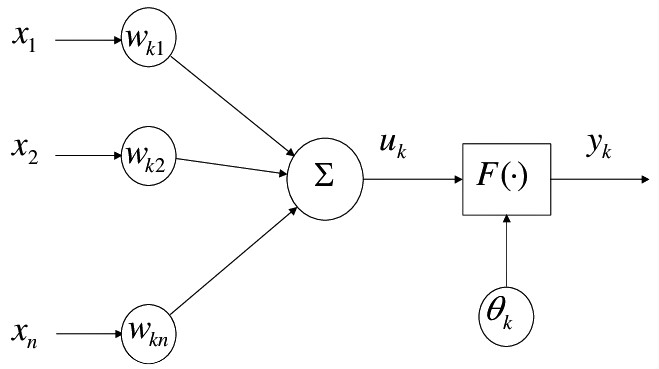
\includegraphics[scale=0.5]{1.jpg}
    \caption{Estructura de un neurona artificial.}
    \label{fig:mesh1}
\end{figure}

La red aprende examinando los registros individuales, generando una predicción para cada registro y realizando ajustes a las ponderaciones cuando realiza una predicción incorrecta. Este proceso se repite muchas veces y la red sigue mejorando sus predicciones hasta haber alcanzado uno o varios criterios de parada. Al principio, todas las ponderaciones son aleatorias y las respuestas que resultan de la red son, posiblemente, disparatadas. La red aprende a través del entrenamiento. Continuamente se presentan a la red ejemplos para los que se conoce el resultado, y las respuestas que proporciona se comparan con los resultados conocidos. La información procedente de esta comparación se pasa hacia atrás a través de la red, cambiando las ponderaciones gradualmente. A medida que progresa el entrenamiento, la red se va haciendo cada vez más precisa en la replicación de resultados conocidos. Una vez entrenada, la red se puede aplicar a casos futuros en los que se desconoce el resultado.

\begin{figure}[h]
    \centering
    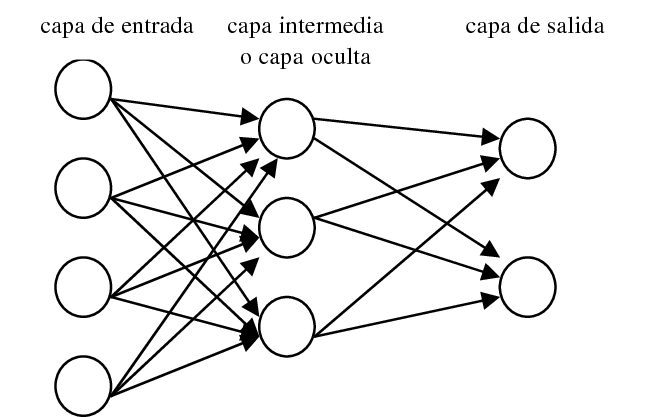
\includegraphics[scale=0.4]{2.png}
    \caption{Estructura de red neuronal.}
    \label{fig:mesh1}
\end{figure}

Saber que arquitectura de red neuronal es la ideal para el caso de estudio es el verdadero reto. Actualmente se cuentan con métodos heuristicos de optimización que pueden ser aplicados en cualquiera de los algoritmos descritos anteriormente. En este caso, al ser dificil de probar multiples combinaciones de capas y neuronas, es mejor implementar una heuristica sencilla para encontrar las combinaciones adecuadas. Una de esas técnicas es conocida como busqueda aleatoria. La búsqueda aleatoria implica generar y evaluar entradas aleatorias a una función objetivo. Se puede generar una muestra aleatoria de un dominio usando un generador de números pseudoaleatorios. Cada variable requiere un límite o rango bien definido y se puede muestrear un valor aleatorio uniforme del rango y luego evaluarlo. La función objetivo puede plantearse como una funcion lineal en combinación con las metricas de evaluación de interes como la exactitud o el F1-score o simplemente usar una de las metricas a maximizar. 

\subsection{Métricas de evaluación}
En el aprendizaje automático la matriz de confusión es una herramienta que permite visualizar el desempeño de un algoritmo  de aprendizaje supervisado. Cada columna de la matriz representa el número de predicciones de cada clase, mientras que cada fila representa a las instancias en la clase real. Nos permite ver  qué tipos de aciertos y errores está teniendo nuestro modelo a la hora de pasar por el proceso de aprendizaje con los datos. EN la matriz de confusión existen 4 resultados posibles: 

\begin{itemize}
\item Verdadero positivo (VP): El valor real es positivo y  la prueba predijo tambien que era positivo. O bien una persona está enferma y la prueba así lo demuestra.
\item Verdadero negativo (VN): El valor real  es negativo y la prueba predijo tambien que el resultado era negativo. O bien la persona no está enferma y la prueba así lo  demuestra.
\item Falso negativo (FN): El valor real es positivo, y la prueba predijo  que el resultado es negativo. La persona está enferma, pero la prueba dice de manera incorrecta que no lo está. Esto es lo que en estadística se conoce como error tipo II
\item Falso positivo (FP): El valor real es negativo, y la prueba predijo  que el resultado es positivo. La persona no está enferma, pero la prueba nos dice de manera incorrecta que silo está.
\end{itemize}

A partir de estas 4 opciones  surgen las métricas de la matriz de confusión:  Por una parte la exactitud y la precisión y por otra la Sensibilidad y la Especificidad. En este trabajo solo se utiliza la exactitud para comprobar la efectividad del algoritmo. Esa métrica se refiere a lo cerca que está el resultado de una medición del valor verdadero. Se representa como  la proporción de resultados verdaderos (tanto verdaderos positivos como verdaderos negativos) dividido entre el número total de casos examinados (verdaderos positivos, falsos positivos, verdaderos negativos, falsos negativos). 

\begin{equation}
exactitud=\frac{VP+VN}{VP+FP+FN+VN}
\end{equation}

\section{Resultados}
Para realizar la práctica se programó en lenguaje Python los dos sistemas de regresión. Primero se obtuvo el conjunto de datos publico Dry Bean Dataset el cual contiene información de 7 distintos tipos de fijoles como se muestra en la Tabla 1. Se tuvo que hacer un pre-procesamiento de los datos debido las clases son categoricas y los datos se normalizaron (ver anexo A). los datos se dividieron para entrenamiento y pruebas en una proporcion 80/20 respectivamente.\\

Con los datos pre-procesados se entrenaron los algoritmos mencionados en la sección anterior con los siguientes parametros: 
\begin{itemize}
\item KNN 
\begin{itemize}
\item valor k=5
\item distancia euclidiana
\end{itemize}
\item Árbol de desición 
\begin{itemize}
\item Criterio de homogeneidad: gini/entropía
\end{itemize}
\item Bosques aleatorios
\begin{itemize}
\item Número de árboles: 10
\end{itemize}
\item SVM
\begin{itemize}
\item kernel: función de base radial 
\end{itemize}
\end{itemize}

Para definir el número de capas ocultas de la red neuronal, el número de neuronas por capa, el ratio de aprendizaje y el optimizador se hace uso de la libreria keras-tuner que cuenta con el método de busqueda aleatoria. La función objetivo se elige como la exactitud y se definieron los siguientes valores como área de busqueda: 

\begin{itemize}
\item Número de capas ocultas: entre 0 y 8 
\item Número de neuronas por capa: entre 16 y 256
\item Valor de ratio de aprendizaje: entre $1e^{-4}$ y $1e^{-2}$
\item Optimizadores: Adam y Stochastic Gradient Descent
\end{itemize} 

Los valores que finalmente resultaron optimos de la busqueda fueron: 
\begin{itemize}
\item Número de capas ocultas: 7 
\item Número de neuronas por capa: 124
\item Valor de ratio de aprendizaje: 0.00055
\item Optimizadores: Adam 
\end{itemize} 

\begin{table}[H]
\begin{center}
\begin{tabular}{| c | c |}
\hline
\multicolumn{2}{ |c| }{Dry-Bean dataset} \\ \hline
Dato & Descripción \\ \hline
Área & El área de una zona de frijol \\ \hline
Perímetro & La longitud de su borde \\ \hline
Longitud del eje mayor & Distancia más larga entre los extremos \\ \hline
Longitud del eje menor & Línea más larga con el frijol \\
& perpendicular al eje \\ \hline
Relación de aspecto & Relación entre las longitudes  \\ \hline
Excentricidad  & Excentricidad de la elipse   \\ \hline
Área convex & Píxeles en el polígono convexo \\ 
& más pequeño  \\ \hline
Diámetro equivalente & Diámetro que tiene la misma área \\
& que un frijol \\ \hline
Extensión & Relación de los píxeles delimitadores al \\
& área del frijol \\ \hline
Solidez  & relación píxeles capa convexa y dentro \\
& de los frijoles \\ \hline
Redondez  & Calculando $\frac{4piA}{P^2}$ \\ \hline
Compacidad  & Mide la redondez de un objeto $\frac{Ed}{L}$ \\ \hline
Factor de forma 1 &  SF1 \\ \hline
Factor de forma 2 &  SF2 \\ \hline
Factor de forma 3 &  SF3 \\ \hline
Factor de forma 4 &  SF4 \\ \hline
Clase & (Seker, Barbunya, Bombay, Cali, Dermosan, \\
& Horozy Sira) \\ \hline
\end{tabular}
\caption{conjunto de datos Dry-Bean }
\end{center}
\end{table}

Los resultados de los experimentos se pueden observar en la Tabla 2 

\section*{Conclusiones}
Como se pudo observar en los resultados, los bosques aleatorios son más robustos que la regresión lineal multiple aunque requiere más tiempo de procesamiento. Sin embargo, actualmente el poder de computo es cada vez mayor por lo que el tiempo se reduce con el paso de los años mediante el hardware. Durante el entrenamiento no se tomó en cuenta la variable categorica del modelo del auto ya que al intentar convertirla en variable dummy, eran demasiadas variables que no podian ser procesadas. Para trabajo futuro se puede modificar manualmente el conjunto de datos para asegurarse en reducir esa variable y colocar solo la marca del vehiculo. No se realizó en este trabajo ya que el rendimiento obtenido es considerablemente optimo por lo que podría no valer la pena incluir esas variables dummies. 

Las regresiones no son 100\% efectivas ya que no siempre se va a ajustar perfectamente a los valores a predecir pero si se puede hacer una aproximación cercana mediante la optimización de parametros de los métodos. Ademas, es bueno revisar de ser posible los datos que se proporcionan para el entrenamiento y eliminar los valores atipicos para evitar errores. El sobreajuste es un problema que trata de evitar los bosques aleatorios y que generalmente cumple su función, pero dependiendo de la aplicación puede optarse por una técnica u otra. A pesar de no ser confiables en su totalidad. las predicciones que es capaz de realizar alguno de estos métodos son lo suficientemente robustos para utilizarse en la industria ajustando el modelo lomejor posible para mejores resultados. 


\begin{thebibliography}{00}
\bibitem{b1}Yang, Q. (2017). Regression. In: Schintler, L., McNeely, C. (eds) Encyclopedia of Big Data. Springer, Cham. https://doi.org/10.1007/978-3-319-32001-4-174-1.
\bibitem{b2} Probabilidad y estadística aplicadas a la ingeniería, Douglas C. Montgomery y George C. Runger. Limusa Wiley, 2002. Segunda edición.
\bibitem{b3} Rokach, L., Maimon, O. (2005). Decision Trees. In: Maimon, O., Rokach, L. (eds) Data Mining and Knowledge Discovery Handbook. Springer, Boston, MA. https://doi.org/10.1007/0-387-25465-X-9.
\bibitem{b4} Cutler, A., Cutler, D.R., Stevens, J.R. (2012). Random Forests. In: Zhang, C., Ma, Y. (eds) Ensemble Machine Learning. Springer, Boston, MA. https://doi.org/10.1007/978-1-4419-9326-7-5.

\end{thebibliography}

\section{Anexo A}
Lectura de conjunto de datos y separandolos en variables dependientes e independientes y eliminación de valores incompletos.  
\lstset{language=Python, breaklines=true, basicstyle=\footnotesize}
\lstset{numbers=left, numberstyle=\tiny, stepnumber=1, numbersep=-2pt}
\begin{lstlisting}[frame=single]
    cols=["MPG", "cylinders", "displacement", "horsepower", "weight", "acceleration", "model year", "origin"]
    dataset=pd.read_csv("auto-mpg.data", na_values="?", comment='\t', sep=' ', skipinitialspace=True, names=cols)
    X=dataset.iloc[:,1:].values
    Y=dataset.iloc[:,0].values
\end{lstlisting}

Normalizado de datos. 
\begin{lstlisting}[frame=single]
    sc=StandardScaler()
    X=sc.fit_transform(X)
\end{lstlisting}

Separando el conjunto de datos.
\begin{lstlisting}[frame=single]
    X_train, X_test, Y_train, Y_test=train_test_split(X,Y,test_size=0.2, random_state=0)
\end{lstlisting}

\subsection{Regresión lineal multiple}

Ejecución de la regresión lineal multiple y calculo de las metricas de evaluación. 
\begin{lstlisting}[frame=single]
    regresion=LinearRegression()
    regresion.fit(X_train, Y_train)
    ypred=regresion.predict(X_test)

    print("R^2 : ", r2_score(Y_test, ypred))
    print("R^2 ajustada: ", 1 - (1-r2_score(Y_test, ypred))*(len(Y)-1)/(len(Y)-X.shape[1]-1))
\end{lstlisting}

\subsection{Bosques aleatorios}
Ejecución del bosque aleatorio estableciendo 10 árboles y calculo de las metricas de evaluación. 
\begin{lstlisting}[frame=single]
    regresion=RandomForestRegressor(n_estimators=10 ,random_state=0) 
    regresion.fit(X_train, Y_train)
    ypred=regresion.predict(X_test)
    
    print("R^2 : ", r2_score(Y_test, ypred))
    print("R^2 ajustada: ", 1 - (1-r2_score(Y_test, ypred))*(len(Y)-1)/(len(Y)-X.shape[1]-1))

\end{lstlisting}
\end{document}